%
%===============>>  ГРУППА 8-1 МОДУЛЬ 7  <<=============
%
\setmodule{7}

%BEGIN_FOLD % ====>>_____ Занятие 1 _____<<====
\begin{class}[number=1]
	\begin{listofex}
		\item Занятие 1
	\end{listofex}
\end{class}
%END_FOLD

%BEGIN_FOLD % ====>>_____ Занятие 2 _____<<====
\begin{class}[number=2]
	\begin{listofex}
		\item В прямоугольном треугольнике два катета равны \( 3 \) и \(  4 \). Найдите гипотенузу.
		\item Катеты прямоугольного треугольника равны \( 5 \) и \( 12 \). Чему равна гипотенуза?
		\item В прямоугольном треугольнике гипотенуза равна \( 20 \), а один из катетов равен \( 12 \). Чему равен другой катет?
		\item В прямоугольном треугольнике один из катетов равен \( 8 \), гипотенуза этого треугольника равна \( 17 \). Чему равен второй катет?
		\item Катет прямоугольного треугольника равен \( 7 \), а гипотенуза равна \( 25 \). Найдите длину второго катета.
		\item В равнобедренном прямоугольном треугольнике гипотенуза равна  \( 14\sqrt{2} \). Найдите длину катетов.
		\item Основание равнобедренного треугольника равно \( 16 \), боковая сторона равна \( 10 \). Чему равна высота проведенная к основанию этого треугольника?
		\item Боковая сторона равнобедренного треугольника равна \( 13 \), а длина основания равна \( 10 \). Найдите площадь этого треугольника.
		\item Найдите высоты равностороннего треугольника, если известно, что его сторона равна \( 8\sqrt{2} \).
		\item Дан параллелограмм \( ABCD \), где \( AB=15 \), \( AD=9 \). Также известно, что высота из точки \( B \) к основанию \( AD \) падает на точку \( D \). Чему равна площадь параллелограмма?
		\item Диагонали ромба равны \( 12 \) и \( 16 \) см. Чему равен периметр? Чему равна площадь? 
		\item Найдите все углы параллелограмма, если сумма двух из них равна \( 100^{\circ}\).
		\item В параллелограмме биссектриса угла \( А \) делит сторону \( ВС  \) на отрезки, равные \( 3 \) и \( 5  \) см. Найдите его периметр.
		\item Найдите углы параллелограмма, зная, что один из них больше другого на \( 50^{\circ} \).
	\end{listofex}
\end{class}
%END_FOLD

%BEGIN_FOLD % ====>>_ Домашняя работа 1 _<<====
\begin{homework}[number=1]
	\begin{listofex}
		\item Домашняя работа 1
	\end{listofex}
\end{homework}
%END_FOLD

%BEGIN_FOLD % ====>>_____ Занятие 3 _____<<====
\begin{class}[number=3]\begin{definit}
		\textbf{Синусом} острого угла прямоугольного треугольника называется отношение противолежащего катета к гипотенузе.
	\end{definit}
	\begin{definit}
		\textbf{Косинусом} острого угла прямоугольного треугольника называется отношение прилежащего катета к гипотенузе.
	\end{definit}
	\begin{listofex}
		\item В треугольнике \( ABC \) угол \( C \) равен \( 90 \) градусов, \( AC=6 \), \( AB=20 \). Найдите \( \sin B \).
		\item  В треугольнике \( ABC \) угол \( C \) равен \( 90 \) градусов, \( BC=9 \), \( AB=20 \). Найдите \( \cos B \).
		\item Найдите синус, косинус углов \( A \) и \( B \) треугольника \( ABC \) с прямым углом \( C \), если:
		\begin{tasks}(2)
			\task \( BC=8 \), \( AB=17 \)
			\task \( BC=21 \), \( AC=20 \)
			\task \( BC=1 \), \( AC=2 \)
		\end{tasks}
		
		\item В треугольнике \( ABC \) угол \( C \) прямой, \( BC=8 \), \( \sin A=0,4 \). Найдите \( AB \).
		\item В треугольнике \( ABC \) угол \( C \) прямой, \( AC=15 \), \( \cos A=\dfrac{5}{7} \). Найдите \( AB \).
		\item В треугольнике \( ABC \) угол \( C \) равен \( 90\degree \), \( BC=12 \), \( \sin A=\dfrac{4}{11} \). Найдите \( AB \).
		\item Катеты прямоугольного треугольника равны \( \sqrt{15} \) и \( 1 \). Найдите синус наименьшего угла этого треугольника.
		\item В треугольнике \( ABC \) угол \( C \) равен \( 90\degree \), \( \sin A=\dfrac{4}{5} \), \( AC=9 \). Найдите \( AB \).
		\item  Есть прямоугольный треугольник \( ABC \), где \( \angle C=90^{\circ} \), и \( AC=7 \), \( AB=25 \). Найдите длину \( BC \).
		\item Сумма двух углов параллелограмма равна \( 62^{\circ} \). Найдите один из оставшихся углов. Ответ дайте в градусах.
		\item Две стороны параллелограмма относятся как \( 9:11 \), а периметр его равен \( 40 \). Найдите большую сторону параллелограмма.
	\end{listofex}
\end{class}
%END_FOLD

%BEGIN_FOLD % ====>>_____ Занятие 4 _____<<====
\begin{class}[number=4]
	\begin{listofex}
		\item 
		\begin{minipage}[t]{\bodywidth}
		Найдите синус и косинус угла AOB, изображенного на рисунке.
	\end{minipage}
	\hspace{0.02\linewidth}
	\begin{minipage}[t]{\picwidth}
		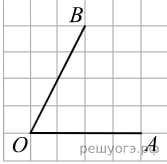
\includegraphics[align=t, width=\linewidth]{\picpath/G81M7L4-1}
	\end{minipage}
	\item Найдите синус, косинус углов \( A \) и \( B \) треугольника \( ABC \) с прямым углом \( C \), если:
	\begin{tasks}(2)
		\task \( BC=4 \), \( AB=12 \)
		\task \( BC=3 \), \( AC=5 \)
		\task \( BC=13 \), \( AC=24 \)
	\end{tasks}
	\end{listofex}
		\begin{definit}
			\textbf{Основное тригонометрическое тождество }
			\begin{tasks}(3)
				\task[]
				\task[] \( \sin ^{2} x+\cos ^{2} x=1  \)
				\task[]
			\end{tasks} 
		\end{definit}
		\begin{listofex}[resume]
		\item Найдите:
		\begin{tasks}(2)
			\task \( \sin\alpha \), если \( \cos\alpha=\dfrac{1}{2} \)
			\task \( \cos\alpha \), если \( \sin\alpha=\dfrac{\sqrt{3}}{2} \)
		\end{tasks}
		\item Вычислить \( \sin \alpha \), если \( \cos \alpha =\dfrac{3}{5}^{\circ} \)	и \( 0 < \angle < \dfrac{\pi}{2} \).
		\item В треугольнике \( ABC  \) угол \( C \) равен \( 90^{\circ} \), \( \sin B = \dfrac{4}{15} \) , \( AB=45 \). Найдите \( AC \).
		\item В треугольнике \( ABC \) угол \( C \) прямой, \( AC=18 \), \( \cos A=\dfrac{6}{13} \). Найдите \( AB \).
		\item В треугольнике \( ABC \) угол \( C \) равен \( 90^{\circ} \), \( AC  =  4 \),  \(  \cos A = 0,5 \). Найдите \( AB \).  
		\item Катеты прямоугольного треугольника равны \( 4\sqrt{6} \) и 2. Найдите синус наименьшего угла этого треугольника.
		\item Найдите синус и косинус  большего острого угла прямоугольного треугольника с катетами \( 7 \) см и \( 24  \) см.
		\item Периметр равнобедренного треугольника равен \( 64 \) см, косинус угла при основании равен \( 0,6 \). Найдите площадь треугольника.
		\item В равнобедренном треугольнике \( ABC \) с основанием \( AB \) боковая сторона равна \( 16\sqrt{15} \),  \( \sin\angle BAC=0,25 \). Найдите длину высоты \( AH \).
		\item Площадь параллелограмма равна \( 40 \), а две его стороны равны \( 5  \) и \( 10 \). Найдите его высоты.
	\end{listofex}
\end{class}
%END_FOLD

%BEGIN_FOLD % ====>>_ Домашняя работа 2 _<<====
\begin{homework}[number=2]
	\begin{listofex}
		\item В треугольнике \( ABC \) угол \( C \) прямой, \( BC=12 \), \( \sin A=\dfrac{6}{13} \). Найдите \( AB \).
		\item В треугольнике \( ABC \) угол \( C \) прямой, \( BC=15 \), \( \cos B=\dfrac{18}{30} \). Найдите \( AB \).
		\item  В параллелограмме \( ABCD \) \( CH \) – высота, \( AB = 4 \), \( \cos C = 0,8 \). Найдите \( CH \).
		\item  В треугольнике \( ABC \) \( AB = BC = 10 \), \( \sin A = 0,2 \). Найдите \( AC \).
		\item Вычислить \( \cos \alpha \), если \( \sin \alpha =\dfrac{12}{13}\).Угол \( \alpha \) острый.
		\item  Высота треугольника равна \( 10 \) и образует с прилежащими сторонами углы \( 45\degree \) и \( 60\degree \). Найдите стороны треугольника.
	\end{listofex}
\end{homework}
%END_FOLD

%BEGIN_FOLD % ====>>_____ Занятие 5 _____<<====
\begin{class}[number=5]
	\begin{listofex}
		\item Решите уравнение 
		\begin{tasks}(2)
			\task \( 10 (x-9) =7 \)
			\task \( 2-3(2x+2)=5-4x \)
			\task \( 3x + 5 +(x+5) = (1-x) + 4 \)
			\task \( \dfrac{x-4}{x-6} =2 \)  
			\task \( \dfrac{ 10}{x+6} =1.  \) 
			\task \( \dfrac{6}{x+8} = - \dfrac{3}{4}\) 
			\task \( \dfrac{ x-14}{x-8} = \dfrac{7}{10} \)
			\task \( \dfrac{3}{x-19} =  \dfrac{19}{x-3}  \)
		\end{tasks} 
		\item В треугольнике \( ABC\) \( \angle C = 90\degree \), \(  AB = 1 \), \( BC = 5 \). Найдите \( \sin B \), \( \cos B \).
		\item  Треугольник \( ABC \) прямоугольный, \( AC = 3 \),  \( \sin B = 0,6 \).  Найдите \(AB, BC \).
		\item Треугольник \( ABC \)  \( AB = 15 \), \( \cos B = 0,6 \). Найдите \( AC, BC \).
		\item В треугольнике \( ABC \) угол \( C \) равен \( 90° \),  \( \cos A =  \dfrac{7}{25} \).  Найдите  \( \cos B \).
		\item Дан прямоугольный треугольник \( MNK \) с гипотенузой \( MN \). Найдите \( \cos⁡\angle N \), если \( \sin⁡\angle M=0,8 \).
		\item В треугольнике \( ABC \) \( \angle C=90\degree \) \( \sin\angle BAC=\dfrac{2}{3} \). Найдите \( AC \), если \( AB=6\sqrt{5} \).
		\item Дан прямоугольный треугольник \( ABC \), причем \( \angle C=90\degree \). Известно, что \( \cos⁡\angle B=13 \), \( AB=9 \). Найдите \( BC \).
		\item В параллелограмме \( ABCD \) диагональ \( AC \) в \( 2 \) раза больше стороны \( AB \) и \( \angle ACD=169\degree \). Найдите меньший угол между диагоналями параллелограмма. Ответ дайте в градусах.
		\item В треугольнике \( ABC \) известно, что \( AC=BC=27 \), \( AH  \) – высота, \( \cos\angle BAC=\dfrac{2}{3} \). Найдите \( BH \).
		\item Разность углов, прилежащих к одной стороне параллелограмма, равна \( 40\degree \). Найдите меньший угол параллелограмма. Ответ дайте в градусах.
		\item Высота \( BH \) ромба \( ABCD \) делит его сторону \( AD \) на отрезки \( AH  =  5 \) и \( HD  =  8 \). Найдите площадь и периметр ромба.
		\item Сторона ромба равна \( 5 \), а диагональ равна \( 6 \). Найдите площадь ромба.
	\end{listofex}
\end{class}
%END_FOLD

%BEGIN_FOLD % ====>>_____ Занятие 6 _____<<====
\begin{class}[number=6]
	\begin{listofex}
		\item Решите уравнение:
		\begin{tasks}(2)
			\task \( \dfrac{42}{x^{2}+5x}=\dfrac{7}{x} \)
			\task \( 7x + 8 +(2x+3) = (2-x) + 8 \)
			\task \( \dfrac{x+4}{x-2}=5 \)
			\task \( \dfrac{x-1}{x}=-\dfrac{1}{3} \)
		\end{tasks}
		\item В треугольнике \(ABC \angle C = 90\degree \), \( AC = 6 \), \( \cos A = 0,3 \). Найдите \( AB \), \( BC \).
		\item Найдите синус наименьшего угла треугольника если один катет равен \( 4\sqrt{2} \), а другой \( 2 \) .
		\item 
		\begin{minipage}[t]{\bodywidth}
			Найдите гипотенузу \( AB \) катет \( BC \) по данным рисунков.
		\end{minipage}
		\hspace{0.02\linewidth}
		\begin{minipage}[t]{\picwidth}
			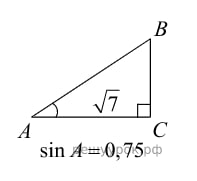
\includegraphics[align=t, width=\linewidth]{\picpath/G81M7L6-2}
		\end{minipage}
		\item \begin{minipage}[t]{\bodywidth}
			Найдите синусы и косинусы углов \( B \) и \( C \).
		\end{minipage}
		\hspace{0.02\linewidth}
		\begin{minipage}[t]{\picwidth}
			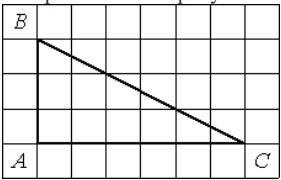
\includegraphics[align=t, width=0.8\linewidth]{\picpath/G81M7L6-4}
		\end{minipage}
		\item В треугольнике \( ABC \) угол \( C \) прямой,
		\( AC=6 \), \( \cos A=0,6 \). Найдите \( AB \).
		\item В треугольнике \( ABC \) угол \( C \) равен \( 90\degree \), \( \sin A=\dfrac{4}{5} \), \( AC=9 \). Найдите \( AB \).
		\item В прямоугольном треугольнике \( ABC \) \( \angle C=90\degree \) \( \cos B=\dfrac{2}{7} \), \( AC=21 \). Найдите \( AB \).
		\item В прямоугольном треугольнике \( MNK \) \( \angle N = 90\degree \), \( \sin M = 0,6 \), \( MN=9 \). Найдите длину \( NK \).
		\item 
		\begin{minipage}[t]{\bodywidth}
			Найдите площадь треугольника, изображённого на
			рисунке.
		\end{minipage}
		\hspace{0.02\linewidth}
		\begin{minipage}[t]{\picwidth}
			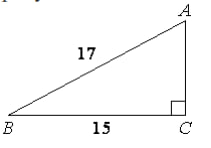
\includegraphics[align=t, width=\linewidth]{\picpath/G81M7L6-3}
		\end{minipage}
	\end{listofex}
\end{class}
%END_FOLD

%BEGIN_FOLD % ====>>_ Домашняя работа 3 _<<====
\begin{homework}[number=3]
	\begin{listofex}
		\item Домашняя работа 3
	\end{listofex}
\end{homework}
%END_FOLD

%BEGIN_FOLD % ====>>_____ Занятие 7 _____<<====
\begin{class}[number=7]
	\title{Подготовка к проверочной}
	\begin{listofex}
		\item Занятие 7
	\end{listofex}
\end{class}
%END_FOLD

=%BEGIN_FOLD % ====>>_ Проверочная работа _<<====
\begin{exam}
	\begin{listofex}
		\item Проверочная
	\end{listofex}
\end{exam}
%END_FOLD

%BEGIN_FOLD % ====>>_ Консультация _<<====
\begin{consultation}
	\begin{listofex}
		\item Постройте график \( y=|x| \) и определите: 
		\begin{tasks}(1)
			\task Промежутки возрастания функции;
			\task Промежутки убывания функции;
			\task Область определения функции;
			\task Область значений функции.
		\end{tasks}
		\item Постройте график \( y=-|x| \) и определите: 
		\begin{tasks}(1)
			\task Промежутки возрастания функции;
			\task Промежутки убывания функции;
			\task Область определения функции;
			\task Область значений функции.
		\end{tasks}
		\item Постройте график \( y=|x|-3 \)
	\end{listofex}
	\newpage
	\title{Домашняя работа}
	\begin{listofex}
		\item Постройте график \( y=|x|+1 \)
	\end{listofex}
\end{consultation}
%END_FOLD
%BEGIN_FOLD % ====>>_ Консультация _<<====
\begin{consultation}
	\begin{listofex}
		\item  На одном из рисунков изображена гипербола. Укажите этот рисунок.
		\begin{tasks}(2)
			\task\begin{minipage}[t]{\picwidth}
				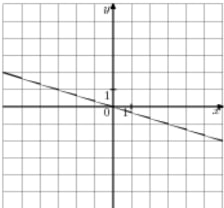
\includegraphics[align=t, width=1.5\linewidth]{\picpath/MoisenkoConsultation17.03-1}
			\end{minipage}
			\task\begin{minipage}[t]{\picwidth}
				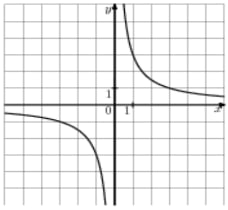
\includegraphics[align=t, width=1.5\linewidth]{\picpath/MoisenkoConsultation17.03-2}
			\end{minipage}
			\task\begin{minipage}[t]{\picwidth}
				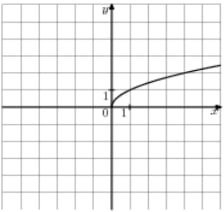
\includegraphics[align=t, width=1.5\linewidth]{\picpath/MoisenkoConsultation17.03-3}
			\end{minipage}
			\task\begin{minipage}[t]{\picwidth}
				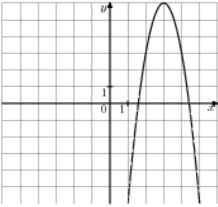
\includegraphics[align=t, width=1.5\linewidth]{\picpath/MoisenkoConsultation17.03-4}
			\end{minipage}
		\end{tasks}
		\item Постройте график функции \( y=-\dfrac{4}{x} \).
		\item Найдите точку пересечения графиков \( y=\dfrac{4}{x} \) и \( y=2 \) 
		\item Постройте график функции \( y = \dfrac{11}{x}+2 \)
		\item Постройте график функции \( y = \dfrac{7+2x}{x}+5 \).
		\item  Какая из указанных точек принадлежит графику функции \( y = -\dfrac{8}{x} \)?\begin{tasks}(3)
			\task \( A (1;8) \) 
			\task \(  B (-1;-8) \)
			\task \( C (1 ; -8) \) 
		\end{tasks} 
		\item Постройте график функции  \(y=\dfrac{ 2x+1}{2x^{2}+x} \).
	\end{listofex}
\end{consultation}
%END_FOLD